\begin{savequote}[75mm]
The best way to have a good idea is to have a lot of ideas. 
\qauthor{Linus Pauling}
\end{savequote}

\chapter{Introduction}
\label{introduction}


\section{Proteins}
\newthought{Proteins are nature’s nano-machines---} they perform the majority of incredibly diverse functions life needs to exist.  A protein's function can be as simple as binding to another protein through an interface [ref], or can be extremely complex, such as working in concert with dozens of other proteins to create gradients of protons across a membrane [ref]. Since they development of next-generation sequencing [ref], we have learned much about protein diversity across the many kingdoms of life---a widely used database Uniref currently contains almost 200,000,000 million different protein sequences [ref]. While there is an incredible amount of information regarding proteins, there is still an incredible amount of we do not yet understand about how they function. 

We are still in the early days of understanding proteins. A database Pfam \cite{Punta2012TheDatabase.} has collected over 17,929 families of proteins as of 2019\cite{El-Gebali2019The2019}. At this point, over 4,000 of those families have no known function. Furthermore, our ability to predict the function of a single mutation remains poor; while there has been recent progress using deep alignments and neural networks {Ingraham}, these methods rely on a deep phylogeny which is not always available. These methods also only are capable of making estimates and do not provide a way of testing the measurements that keep pace at the scale of their predictions. In order to test the predictions, we need new methods of measurement. 

As sequencing improves, we are also beginning to understand the diversity of the human genome, and the effect that has with regards to human protein sequence diversity [ref]. When is a mutation to a protein sequence disease causing, and when is it neutral is something we desperately need to understand as we enter the age of precision medicine. While there has been much progress in this direction, we increasingly realize that we need more data (in the form of genomes sequence) to understand the complexity of 6 billion base pairs of possible variation within the human genome. 

Furthermore, as our ability to understand proteins has improved, they have been increasingly relied on as a modality in medicine. What initially started as harnessing monoclonal antibodies (ref) has led to us engineering gene therapies which hijack a virus of interest, load it with therapeutic cargo in the form of a gene sequence with some therapeutic effect, and deliver it into a cell population to be expressed. While we have come a long way in our abilities in medicine, there are still many hurdles to overcome if we are to continue progress in treating currently incurable disease. 

\begin{figure}[t!]
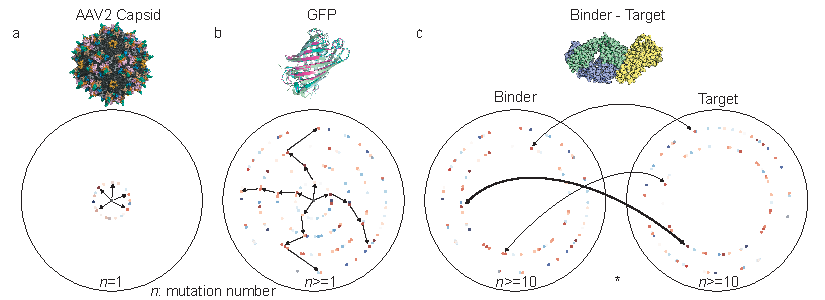
\includegraphics[width=\textwidth]{figures/20190612_x03_landscape_walks.pdf}
\caption[Overview of protein measurement methodologies]{\textbf{Overview of protein measurement methodologies}(A) Using AAV, all possible single mutations are measured to the AAV2 Capsid sequence, and assayed across various functions. (B) using GFP, random mutations are added to differing distances from the starting point, measured in high throughput, and used to walk the landscape to distant points. (C) Using binder modalities and target libraries, libraries of different target proteins are scanned against binding domains with dozens of variable positions, in an effort to learn a global map of interaction ]
\label{fig:Figure 0.0}}
\end{figure}

Engineering proteins to perform functions of interest has been the primary way we have created these new classes of protein therapeutics. Initially, and for the most part still today, this is an inherently random process. For instance, phage display--- a method commonly used to discover antibody fragments which bind potentially relevant therapeutic targets--- involves randomizing the surface variable regions (VR) of an antibody and panning them against a target of interest to find ones which binding. Directed evolution--- a method used from everything from making enzymes with novel functions to altering the tropism of viral capsids---involves subjecting a gene sequence to amplification by an error prone polymerase, then selecting for “errors” in the sequence which create the novel function of interest. While these methods have been incredibly powerful, they have many downsides which will be further addressed below. 

My thesis will aim to answer three main questions, using three different systems. First; what can we learn by making all possible single mutations to a well-studied protein sequence (Fig 1a)For this question, I leveraged the AAV2 capsid {ref}. Second, what can we learn about protein structure from making many mutations to a protein sequence, and furthermore, is there structure to these mutation patterns which we can learn using a statistical model (Fig. 1b). For this question, I used the well-established GFP protein as a model system. And finally, what sort of global structure protein-protein interaction interfaces can we learn from measuring billions of possible interactions(Fig. 1c). In this introduction I will go over these three systems in detail and explain how together, lead us towards the goals of comprehensive protein understanding, and thus ability to perform sophisticated protein design. 

\section{General methods for understating proteins}

Mutagenesis\\
Making single point mutations, or totally random mutations, is the initial way with which we were able to understand proteins. By swapping amino acids at specific positions, we have been able to learn much about proteins functionality, active sites where reactions are catalyzed by proteins etc. This method is incredibly valuable, but also slow and costly, as each mutation must be made individually. 
Alanine scanning is essentially another form of mutagenesis where each position in a protein is replaced by alanine. This enables slightly more functional information to be gleaned in regards to the entire structure of the protein, yet is still relatively slow and costly.

Deep sequencing\\
Sequencing using high-throughput approaches such as Illumina has enabled us to further glean more information about proteins and proteins structure. This has come through completely unbiased sequencing of whole genomes/metagenomes---which has enabled us to learn about the strcuture within protein phylogeny---to making libraries of proteins with mutations and sequencing to determine functionality. While one can make many random mutations and sequence, the ability to directly synthesize thousands of DNA sequences at once has enabled a new era of testing specific designs [ref some stuff]. 

Chip synthesis and targeted design/measurement of proteins\\
Using chip synthesis, we are able to make targeted design of proteins at an extremely parallel scale. This has enabled us to scan protein sequences making many mutations at once [ref shendure fowler], or even make thousands of designs of completely synthetic protein-like moieties [ref baker something]. While incredibly powerful, especially in combination with deep sequencing, the chip synthesis and deep sequencing systems still have drawbacks, which my thesis attempts to develop methods to overcome. The main challenge when using chip synthesis and deep sequencing is the length of DNA elements which can be synthesized or read. Chip synthesis has an upper cap limit at 230 nucleotides, while deep sequencing has some methods which provide long reads [ref pac bio nanopore], there is a trade-off between accuracy and length which makes long reads challenging of one is trying to identify a protein with a single base difference. 

However, we often do now need very long reads to learn all the information contained in a sequence. For instance, if you are to make 1000 single mutations to a protein, this information can be stored in 5 bases of DNA. Levergaing short chains of DNA (termed ``barcodes'') enables one to read out very small sequences and specficially index the mutations associated with that sequence. This methodology has been used in many fields, including MPRA [ref], and has just recently picked up steam in the field of protein measurement. In this thesis, 



\section{AAV: A Promising Vector for Gene Therapy}

AAV has shown promise as a gene therapy vector. There are now two gene therapies approved in the US: Luxturna [ref], which cures a genetic form of blindness, XXXX, which cures babies of spinal muscular atrophy[ref]. Currently, there are XXX active clinical trials using AAV as a gene therapy vector occurring in the US alone. However, some of these clinical trials have failed to meet their endpoints despite promising data on the gene being delivered. This was the case with delivering SERCA2A using AAV for treating heart failure 5 [ref]. It is possible that this disconnect between promising genetic data and lack of efficacy in clinical trials could be due to the specific AAV vectors being used for delivery. This specific trial could have failed because SERCA2A did not have the hypothesized effect or because AAV failed to deliver the gene correctly. The cause of trial failure is still difficult to elucidate, since there is a lack of knowledge regarding how the AAV1 vector performed on its task of transgene delivery. Furthermore, it is estimated that as much as 70\% of the population is immune to AAV through previous exposure, posing large hurdle to therapeutic gene delivery6. Deeper understanding of the AAV capsid will lead to the ability to engineer more efficacious gene therapy vectors.

\begin{figure}[t!]
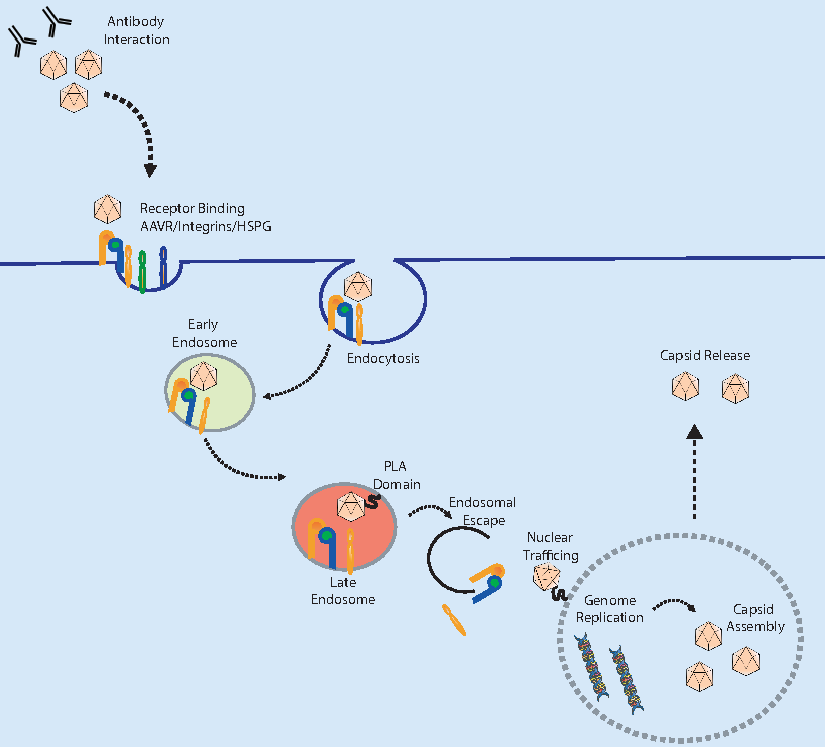
\includegraphics[width=\textwidth]{figures/20190612_aav_cell_diagram.pdf}
\caption[AAV Viral Cycle]{\textbf{AAV Viral Cycle}]
\label{fig:Figure 0.1}}
\end{figure}

The AAV capsid is composed of three proteins: VP1, VP2, and VP3. The VP2 and VP3 proteins are read from internal ribosome binding sites of the VP1/Cap gene7. A complete capsid creates an icosahedral 60mer structure with VP1:VP2:VP3 assembled in a 1:1:10 ratio. VP3 is the only protein needed to form capsid particles and package genomes, while the VP1 subunit is necessary for infection7. Currently, the exact role of VP2 is uncertain. Additionally, new proteins involved in capsid assembly are still being discovered, such as the AAV assembly protein (AAP)8, which is interacts with VP proteins and is thought to facilitate capsid assembly.

During infection, AAV enters the cell through interactions with proteoglycans and surface receptors9,10. It then undergoes clathrin-mediated endocytosis9, during which a conformational change in the VP1 protein occurs that allows it to escape the late endosome (Figure 1)10,11. Intact AAV is shuttled to the nucleus via microtubule trafficking, where capsid disassembly and transcription occurs7. Co-infection with adenovirus activates transcription of Rep proteins and large-scale translation of capsids, enabling the lytic life cycle of AAV and packaging genome-containing capsids7.
    

\section{AAV Capsid Natural Diversity}

There are 12 main genetically distinct serotypes of AAV have been discovered in mice, humans, and non-human primates12. However, in recent years, there has been an explosion of AAV serotypes found from mining DNA from human samples [ref gao]. These 12 serotypes exhibit a broad range of infectivity and mainly differ within hyper-variable regions in exposed loops of the VP3 capsid protein (Figure 2). The exposed loops play important roles in AAV packaging, tropism and neutralization by antibodies of the immune system13-16. Many motifs important in tropism, such as heparin sulfate, sialic acid, and galactose binding regions, are located within hyper-variable regions on the capsid structure17-19. Additionally, certain AAVs cross the blood brain barrier while others cannot; the structural basis for this ability is unknown20. Further understanding of these variable regions remains critical for medical applications of AAV. These regions of variability provide confidence that the AAV vector can be mutated to perform novel functions—a hypothesis that has thus far been investigated through the lens of directed evolution. 

\begin{figure}
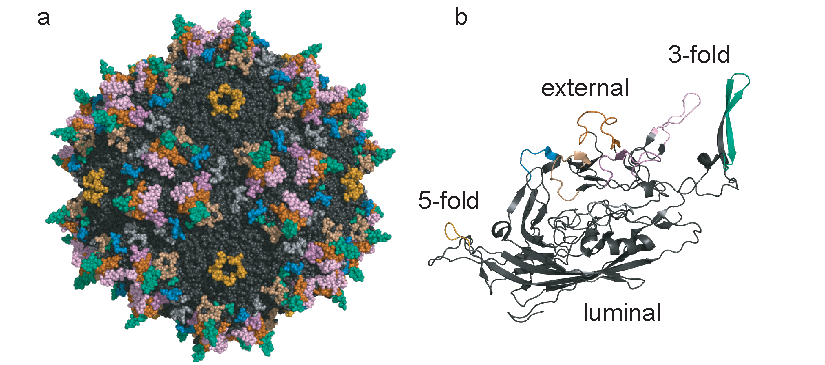
\includegraphics[width=\textwidth]{figures/20190612_viral_capdis_vr.pdf}
\caption[Structure of AAV2]{\textbf{Strcutre of AAV2}
a, AAV2 capsid structure, variable regions highlighted. b, AAV2 monomer structure shown as cartoon]
\label{fig:Figure 0.2}}
\end{figure}

\section{Challenges in AAV Vector Engineering}

Because of its potential for use in gene therapy, many attempts have been made to engineer specific tropism and immune evasion into AAV21. These approaches typically use mutagenesis followed by downstream selective pressure (Figure 3)21. Mutagenesis is the engine used to create variation. Different selection strategies are then used to enrich for specific variants.  After the virus has been put through multiple rounds of selection, the surviving AAVs are sequenced to identify the mutations that have been captured by the selective assay. 

Mutagenesis is generally accomplished through one of three methods. Error-prone PCR can be used to generate single base pair mutations,21 and/or capsid shuffling can be used, where multiple AAV capsid variants are digested and ligated together to make a library of chimeric AAV capsids. Peptide display has also been used to insert small peptides at specific locations throughout the capsid, which may confer some novel phenotype22. 

The resulting capsid libraries are then put through many rounds of selections and sequenced once a product with a specific phenotype is observed. When only the end output of a selection is sequenced, it is hard to understand the evolutionary process that leads to the end phenotype. As engineering focused scientists, we often utilize the evolution engine as a tool without attempting to understand the underlying biology. A method that attempts to quantify the effects of specific mutations across an entire fitness landscape could greatly enhance our understanding of how proteins evolve and diversify.  

\subsection{Massively parallel single-amino acid mutagenesis: A novel approach to understanding AAV}

Recently, a method termed massively parallel single-amino-acid mutagenesis, or scanning saturation mutagenesis (SSM), has been developed to measure the effects of each possible amino acid mutation at every possible position within a protein23-26. This method was used to characterize mutational effect on BRCA1’s function of homology-directed repair, with clinically relevant outcomes{also cite new shendure paper}23. Also novel ligands were engineered to bind LacI through single amino acid mutations24. Surprisingly, residues highly conserved within the LacI phylogeny were found to be tolerant of mutation. Furthermore, work using SSM on infA in E. coli has shown how amino acid properties such as hydrophobicity, size, flexibility, and charge play important roles within different regions of the 3D protein structure26. These studies show the adaptability of SSM across a wide range of proteins as well as the ability to identify functionality in protein regions that were previously poorly understood. 

SSM involves making a library that includes each possible amino acid at every position within a given protein25. This library is then put through functional selections to see which amino acids are enriched. Importantly, both the starting and ending populations are sequenced, which allows for specific quantifications of enrichments across the fitness landscape. However, this type of experimentation has remained challenging due to both difficulty constructing these libraries and difficulty sequencing the pre- and post-selection libraries. Chip-based synthesis and next generation sequencing have solved a lot of these problems; the adaption of these methods to SSM will be further explained in the aims of this proposal.  

Beyond scanning all amino-acids within a protein, one can also scan all possible codons in a protein. This, which I term comprehensive codon scanning (CCS), enables discovery of novel cryptic elements within a gene, plus also determination of the importance of codons used to a protein sequence. A protein’s function can be indirectly effected by the choice of codons used for coding it, and while we understand the importance of this in locations such as the genes n-terminus (cite DBG, kelsic), the effect of codon usage throughout a gene is not fully understood. Furthermore, the AAV2 capsid plays many functional roles, one of which is packaging DNA---methods such as comprehensive codon scanning could help elucidate the importance of such interactions between genome and capsid protein in this case.

Previous studies have investigated the effects that fitness constraining mutations have on AAV’s properties. In 2014, Hidachi et al investigated the effect of double alanine scanning through the VP3 portion of AAV9 and assayed for packaging, infectivity, and antibody neutralization27. This work provided novel fitness information, identifying positional constraints for liver tropism, mutations that completely inhibited packaging, and positions associated with antibody neutralization. Surprisingly, this study also identified alanine mutations that increased liver tropism and speed of clearance from the blood in mice. The work I build on these first steps taken to understand the fitness landscape. By looking at all possible mutations at every position, comprehensively elucidate constraints on packaging and basic infectivity, and also further understand these effects in vivo. Using comprehensive codon scanning, I also discover a new cryptic ORF, termed MAAP. 

While this work shows the importance of understanding the effect of single mutations on protein function, in order to understand proteins at the design level (need to define this), we need to understand what happens when multiple mutations are made to a protein. This is confounded by the fact that mutations can interact, through a process called epistasis, and also the immense complexity that proteins can achieve through multiple mutations. Using the next system, GFP, I aim to understand the complexity of multiple mutations and our ability to predict protein functionality in this more sophisticated regime, using machine learning.

\section{GFP as a model protein for building large datasets of protein fitness}

GFP, since its discovery (ref tsien) has been one of the most important tools in the biological sciences. GFP has enabled us to visualize the components of the micriosopic level, molecular biology is occurring, in a new way. By tagging different proteins with GFP, we have elucidated protein localization, dynamics, and interaction at a new scale. GFP is an incredibly stable protein [ref]. It can fold and perform its function of florescence in a wide array of biological conditions, something which has led to it’s use time and time again across all domains of biological research.

Using the original avGFP (define) as a base, there has been many rounds of improvement to GFP, in terms of brightness stability, and quaternary structure. The original avGFP excitation is at UV wavelength, making it challenging to use in living cells. Through directed evolution, variants such as eGFP were created, which excite with blue light, and are thus more compatible with imaging in live cells, and also brighter. GFP also has the tendency to dimerize under many conditions [ref], and through directed evolution, this ability has also been ablated, leading to monomeric proteins which are less likely to interfere with protein function when used as a fusion. Throughout these evolutionary paths, variants of GFP have been made with dozens of mutations, that maintain, and even increase, the functionality of the original protein. My interest is in understanding these landscapes; if we can understand the different paths that enable these functional gains, it may be possible to engineer them as well. 

The main interest in using GFP for the goal of modeling and understanding multiple mutations is twofold---its size makes it very amenable to NGS, and it functionality makes measuring it’s phenotype very simple. Size is an important constraint when making many mutations to a single protein, primarily due to constraints place by using NGS to measure the mutations made. While NGS is an incredible powerful technology, enabling one to make millions of measurements in a single experiment, the current read lengths are constrained to under 600 base pairs. Thus, pairing mutations outside of a window of this length remains challenging. While there are methods which enable one to do this, starting with a relatively small protein such as GFP makes the pairing of distant mutations easier. Using a protein such as the AAV Capsid gene would be challenging, considering its length is ~2.7 kb.

Second, GFPs function as a fluorescent protein enables one to very easily measure and differentiate between functional and non-functional variants, using fluorescent activated cell sorting (FACS) [ref]. FACS enables us to separate GFPs into different “bins” based on how bright they are and sequencing these bins together. Having an easily determinable functional assay is critical for measuring thousands of variants quickly. Together, these considerations make GFP a good model system for building large datasets to use in downstream machine learning applications. However, many open questions remain in regards to the type and how much information one needs to build a relevant model of a protein fitness landscape. 

\subsection{Generating “interesting” mutational data for models to learn from}

The next consideration for generating interesting mutational data is what type of information one needs to train an interesting model of mutation. In general, when making multiple mutations, mutated residues have the ability to interact through a process known as epistatsis [ref]. Iften these interaction can be deleterious, where both residues are neutral in fitness when considered individually, but when combined together, create some sort of fitness defect. However, there are many types of epistasis, that follow outline below: (outline the types of epistatsi here form poelwjickl paper)

What’s particularly interesting are sign and reciprocal sign epistasis, where one mutation recovers the defect of another, or where two mutations individually both create defects, but together the mutations are stabilized and have a positive effect on protein fitness. Observing these types of mutations is very challenging through a strictly random process, and thus must be selected for through clever sequence manipulation; in this thesis I develop a method to select for these types of interesting mutations for training on, and develop models for understanding their function. 

Importance of data structure in building models capable of generalization 

One further consideration when trying to build models capable of predicting protein fitness is data structure. In the ideal case, we would have all possible sequences for a protein of length n. If we consider GFP, this is 236 amino acid protein, with 20 possible amino acids at each position, this would lead to a complexity of \( 20^{236}\). As this number is essentially impossible for our brain to comprehend, the easiest way to put it if you took the number one trillion, and raised in to the power of 10 (or times a trillion by itself 10 times), you would still be only at 1/3rd of the possible combinations of proteins at this length. 

Of course, the vast majority of these sequences will not have the function of fluorescing. There are strict sequence constraint a protein must maintain in order to fluoresce, notably the chromophore (3 residues which undergo a chemical transformation enable them to emit light when excited by light) and the structure which maintains said chromophore. That being said, there are likely trillions of sequences which satisfy this constraint; an effectively infinite number  when considering our current ability to measure proteins. Furthermore, it is likely that there are many sequences which have no relationship to each other (ie no sequence identity), but still perform the exact same function. We know that there are FPs with ~20\% sequence identity, which maintain the beta-barrel shape of GFP, and fluoresce at very similar wavelengths. Since it is possible to build fluorescent proteins with incredibly different sequences, the question becomes, is it possible to build statistical models which are capable of learning this structure in the data? Chapter 3 of this thesis will build methods towards this understanding. 

\section{Understanding protein-protein interactions using new sequencing and synthesis methods}

The final chapter of my thesis will aim to build methods towards the goals of understanding how proteins interact with each other. This is a particularly challenging problem, due to the complexity I described above being at least squared. Yet, we know that no proteins exists in a vacuum, all proteins by definition must interact with other proteins (be it themselves or other proteins in the cell) and it is through these complex interactions which life is formed.  A method which enables probing interactions between proteins in high throughput would be not only of value to the fundamental research community; the vast majorities of proteins used as therapeutics are antibodies, which main function is to bind another protein in the cell and inhibit its function. Therefore, being able to understand how the interactions occur, and predict them, would be of immense value to therapeutic interventions. My thesis will primarily deal with the interaction of a potential therapeutic binding domain, such as an antibody, with a possible target, such as protein mutated in cancer. However, it is important to understand the challenges with measuring protein-protein interactions from a more global contexts, which outline below.

Methods for understand protein-protein interactions include primarily what are known as “2-hybrids”. Initially developed in yeast [cite stan fields] the general idea is to fuse two potential interacting proteins (one termed “bait”, the other “prey”) to different elements of transcription factors. If the bait and prey indeed do interact, then a transcriptional event occurs, thus creating a measurable signal. This method has been used for the past three decades to help determine if proteins are interacting at the molecular level. 

While the standard 2-hybrid methods have been every useful in the contexts of known proteins fro the human proteome, many challenges in measurement still remain. Initial 2 hybrid screen focused on scanning a “prey” library against a single “bait” target. While this is useful for understanding what protein interacts with a single target, it does not give us comprehensive information of how all proteins interact with each other. Recently, many methods have been developed which enable two libraries of proteins to be screened via the 2-hybrid method (cite roth, baker, ecker). However, even when screening in a library by library format, it is still difficult determine the exact interface of interaction. Since proteins are generally screened in a format where the whole protein is present, the exact interface of interaction is virtually indeterminable. An ideal method would enable one to determine the exact position of binding, while also enable screening of numbers appreciable to build models of protein-protein interactions.

\section{Antibodies and other binding domains: hurdles and opportunities}

One of the most therapeutically important protein interactions is that of an antibody binding its target. Antibody binding is the initial step in a learned immune response which leads to targeted degradation of the protein target and its associated components. This functionality has been leveraged to make research tools and therapeutics  which enable us to bind a protein specifically: an important ability which in research can tell us ``is this protein present’’, and in medicine can enable us to target a specific protein or cell for immune system degradation.

Antibodies have specific regions of variability that are programmed by a recombination process in the immune system [ref]. These regions are known to dictate how the antibody binds to its target. Antibodies which work well are then propagated by the body and leveraged to neutralize a pathogen, or a misfunctioning cell. This ability to generate localized diversity while maintaining constant scaffolding has enabled humans to engineer libraries of synthetic antibodies for screening against protein targets of therapeutic interest.

Initially, antibodies were generated through the hybridoma process [ref]. A mouse or similar animal was injected with an antigen protein of interest, then the B-cells which generate antibodies were purified and screened for binding to the known antigen. Relying on in vivo model to do the heavy lifting of diversity generation is still a common process, however recently many groups use completely synthetic libraries through processes known as phage or yeast display.

In phage display, antibody sequences are created synthetically through molecular cloning methods, and diversity is added at the known variable positions in the form of random nucleotides. These random nucleotides can be skewed to provide speficic distrbutions of amino acids at certain positions in the sequence, to help make the variblity look more like what we see in a human [ref]. The antibody sequence library can then be fused to the surface of a phage or yeast particle (with a linker to link the heavy and light chains), and this library is then screened in vitro against a target protein of interest. Usually this selection process is repeated, with rounds of diversification occasionally added, until a binder of high affinity is found against the antigen. Generally, while both of these processes are capable of delivering binders which bind to a specific antigen, they lack in ability to generate information about how the binding interaction occurs, and also often do not maintain the other properties of interest for utility in the research or therapeutic setting (folding, stability, pharmacokinetics etc). 
In an ideal world, one would be able to generate binders to any sequence on demand, which maintained quality folding properties as well as the in vivo proteins of interest like pharmacokinetics, and target engagement in the relevant context--- ie. on the surface of a cell in the blood as example. Current methods fail at this for a many reasons. 

First, whether you raise an antibody in a mouse or using phage display, you generally are raising that antibody to a specific sequence only. That means any related sequences that may have similar reactivities are ignored. While one can perform negative selections against related sequences, it is still not known if the binding will act similarly in the context of the body. This is further confounded by the fact that some sequences may be distant in sequence space, but take on very similar structural motifs. Therefore, through the lens of just screening on target at a time, it is challenging to understand the landscape of specificity across the possible targets in the body. 

We know that specificity is a quite problematic from a research perspective. It is estimated that 800 million dollars globally is wasted on antibodies of poor quality [ref]. Furthermore, even antibodies from the same provider, but from different lots can have different binding capabilities [ref nature methods mass spec antibody paper]. Whiel there is less data from antibodies which fail clinical trials, it is reasonable to assume that the specificity problem also plagues antibodies here as well. Understanding why this is the case is incredibly important for solving this problem, yet the challenge is the current data strcutures do not provide enough information about antibody sequence for one to understand why. 

In order to understand how an antibody binds a target of interest, we need to generate my examples of antibodies which bind this single target, as well as antibodies which do not. Currently, while the current emthods may provide a few antibodies possible candidate aniytbodies, generally they are then screened one by one, and if they do not work ousdie of the development context, they are discarded. Ideally, we would have thousands to millions of examples of anitbodies which vary in the ability to bind a specific target. From this information, we could build a model the sequence determinant which make an antibody good at binding a specific target, or not. While there has been  some developments towards this ability [ref], we still have much to learn. Furthermore, having this information would need to be complemented by specificity information as well to learn all properties which make a binder have the qualities we want. 

Specificity is more challenging to measure. The challenge comes from the combinatorial explosion of screening against multiple targets. For example, lets say you wanted to screen a phage display antibody library against 100 targets. This would require running 100 individual campaigns, which for a well funded lab may be feasible. Now if we extrapolate that to the entire human proteome, this equates to approximately 20,000 campaigns. Furthermore, if one wishes to understand the specificity of the library across these contexts, all 20,00 of these campaigns would have to be deep sequenced. This type of brute force experimentation, while potentially being effective, is too slow and costly. 

Here is what an ideal method would enable---screening a large library of target proteins against a large library of binding proteins in a single experiment, using deep sequencing to read out which pairs interact. This method would be agnostic to the binding modality which is used (nanobody, antibody or non-standard), as well as the target. Furthermore, the ideal method would provide in depth information regarding the location where it is binding the target protein. Even more ideally, we would understand the specific residues between binding domain and target protein which are interacting. Finally, this interaction would be recapitulative of the interaction in the endogenous relevant context--- whether that is acting in inside a cell or in the blood of an animal. In this thesis, I build toward a system meeting these requirements. 

In summary my thesis will deal with three main concepts: What do we learn when measuring all single mutations to a protein, what can we learn from measuring multiple disperse mutations to a protein, and what can we learn from measuring multiple mutations to two possibly interacting proteins. Using these methods, I show that there is still much to be learned, even from making a single mutation. I then build toward a future where we are empowered by high throughput experimental data to perform measurement driven design of proteins. 

%%%%%%%%%%%%%%%%%%%%%%%%%%%%%%%%%%%%%%%%%%%%%%%%%%%%%
% %\newthought{Proteins are nature’s nano-machines}---they perform the majority of incredibly diverse requirements life needs to exist.  A proteins function can be as simple as binding to another protein through an interface [ref], or can be extremely complex, such as working in concert with dozens of other proteins to create gradients of protons across a membrane [ref]. Since they development of next-generation sequencing [ref], we have learned much about protein sequence across the many kingdoms of life---a widely used database Uniref currently contains almost 200,000,000 million different protein sequences [ref]. While there is an incredible amount of information regarding proteins, there is still so an incredible amount of we do not yet understand about how they function. 

% We are still in the early days of understanding proteins. A database Pfam \cite{Punta2012TheDatabase} has collected over 17,929 families of proteins as of 2019 {gebali}. At this point, over 4,000 of those families have no known function. Furthermore, our ability to predict the function of a single mutation remains poor; while there has been recent progress using deep alignments and neural networks {Ingraham}, these methods rely on a deep phylogeny which is not always available. These methods also only are capable of making estimates and do not provide a way of testing the measurements that keep pace at the scale of their predictions. In order to test the predictions, we need new methods of measurement. 

% As sequencing improves, we are also beginning to understand the diversity of the human genome, and the effect that has with regards to human protein sequence diversity [ref]. When is a mutation to a protein sequence disease causing, and when is it neutral is something we desperately need to understand as we enter the age of precision medicine. While there has been much progress in this direction, we increasingly realize that we need more data (in the form of genomes sequence) to understand the complexity of 6 billion base pairs of possible variation within the human genome. 

% Furthermore, as our ability to understand proteins has improved, they have been increasingly relied on as a modality in medicine. What initially started as harnessing monoclonal antibodies (ref) has led to us engineering gene therapies which hijack a virus of interest, load it with therapeutic cargo in the form of a gene sequence with some therapeutic effect, and deliver it into a cell population to be expressed. While we have come a long way in our abilities in medicine, there are still many hurdles to overcome if we are to continue progress in treating currently incurable disease. 

% Engineering proteins to perform functions of interest has been the primary way we have created these new classes of protein therapeutics. Initially, and for the most part still today, this is an inherently random process. For instance, phage display--- a method commonly used to discover antibody fragments which bind potentially relevant therapeutic targets--- involves randomizing the surface variable regions (VR) of an antibody and panning them against a target of interest to find ones which binding. Directed evolution--- a method used from everything from making enzymes with novel functions to altering the tropism of viral capsids---involves subjecting a gene sequence to amplification by an error prone polymerase, then selecting for “errors” in the sequence which create the novel function of interest. While these methods have been incredibly powerful, they have many downsides which will be further addressed below. 

% My thesis will aim to answer three main questions, using three different systems. First; what can we learn by making all possible single mutations to a well-studied protein sequence? For this question, I leveraged the AAV2 capsid {ref}. Second, what can we learn about protein structure from making many mutations to a protein sequence, and furthermore, is there structure to these mutation patterns which we can learn using a statistical model. For this question, I used the well-established GFP protein as a model system. And finally, what sort of global structure protein-protein interaction interfaces can we learn from measuring billions of possible interactions. 
% In this introduction I will go over these three systems in detail and explain how together, lead us towards the goals of comprehensive protein understanding, and thus ability to perform sophisticated protein design. 

% \section{AAV: A Promising Vector for Gene Therapy}

% AAV has shown promise as a gene therapy vector. There are now two gene therapies approved in the US: Luxturna [ref], which cures a genetic form of blindness, XXXX, which cures babies of spinal muscular atrophy[ref]. Currently, there are XXX active clinical trials using AAV as a gene therapy vector occurring in the US alone. However, some of these clinical trials have failed to meet their endpoints despite promising data on the gene being delivered. This was the case with delivering SERCA2A using AAV for treating heart failure 5 [ref]. It is possible that this disconnect between promising genetic data and lack of efficacy in clinical trials could be due to the specific AAV vectors being used for delivery. This specific trial could have failed because SERCA2A did not have the hypothesized effect or because AAV failed to deliver the gene correctly. The cause of trial failure is still difficult to elucidate, since there is a lack of knowledge regarding how the AAV1 vector performed on its task of transgene delivery. Furthermore, it is estimated that as much as 70\% of the population is immune to AAV through previous exposure, posing large hurdle to therapeutic gene delivery6. Deeper understanding of the AAV capsid will lead to the ability to engineer more efficacious gene therapy vectors.



% The AAV capsid is composed of three proteins: VP1, VP2, and VP3. The VP2 and VP3 proteins are read from internal ribosome binding sites of the VP1/Cap gene7. A complete capsid creates an icosahedral 60mer structure with VP1:VP2:VP3 assembled in a 1:1:10 ratio. VP3 is the only protein needed to form capsid particles and package genomes, while the VP1 subunit is necessary for infection7. Currently, the exact role of VP2 is uncertain. Additionally, new proteins involved in capsid assembly are still being discovered, such as the AAV assembly protein (AAP)8, which is interacts with VP proteins and is thought to facilitate capsid assembly.

% During infection, AAV enters the cell through interactions with proteoglycans and surface receptors 9,10. It then undergoes clathrin-mediated endocytosis 9, during which a conformational change in the VP1 protein occurs that allows it to escape the late endosome (Figure 1) 10,11. Intact AAV is shuttled to the nucleus via microtubule trafficking, where capsid disassembly and transcription occurs7. Co-infection with adenovirus activates transcription of Rep proteins and large-scale translation of capsids, enabling the lytic life cycle of AAV and packaging genome-containing capsids7.

% \section{AAV Capsid Natural Diversity}

% There are 12 main genetically distinct serotypes of AAV have been discovered in mice, humans, and non-human primates12. However, in recent years, there has been an explosion of AAV serotypes found from mining DNA from human samples [ref gao]. These 12 serotypes exhibit a broad range of infectivity and mainly differ within hyper-variable regions in exposed loops of the VP3 capsid protein (Figure 2). The exposed loops play important roles in AAV packaging, tropism and neutralization by antibodies of the immune system13-16. Many motifs important in tropism, such as heparin sulfate, sialic acid, and galactose binding regions, are located within hyper-variable regions on the capsid structure17-19. Additionally, certain AAVs cross the blood brain barrier while others cannot; the structural basis for this ability is unknown20. Further understanding of these variable regions remains critical for medical applications of AAV. These regions of variability provide confidence that the AAV vector can be mutated to perform novel functions—a hypothesis that has thus far been investigated through the lens of directed evolution. 

% \begin{figure}
% 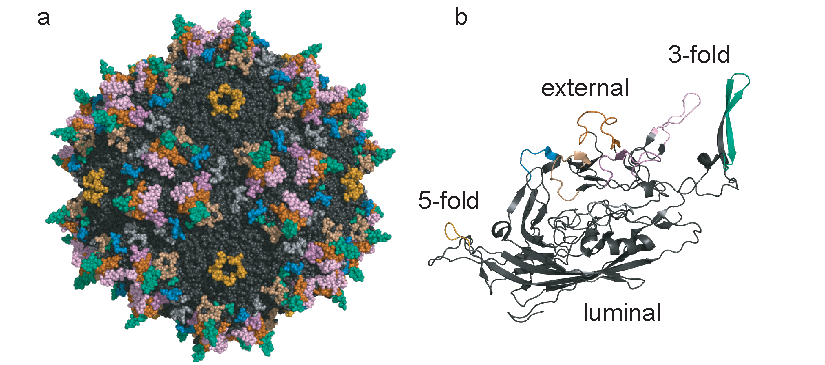
\includegraphics[width=\textwidth]{figures/20190612_viral_capdis_vr.pdf}
% \caption[Structure of AAV2]{\textbf{Strcutre of AAV2}
% a, AAV2 capsid structure, variable regions highlighted. b, AAV2 monomer structure shown as cartoon]
% \label{fig:Figure 0.2}}
% \end{figure}

% section{AAV Vector Engineering - Directed Evolution and its Pitfalls}

% Because of its potential for use in gene therapy, many attempts have been made to engineer specific tropism and immune evasion into AAV21. These approaches typically use mutagenesis followed by downstream selective pressure (Figure 3)21. Mutagenesis is the engine used to create variation. Different selection strategies are then used to enrich for specific variants.  After the virus has been put through multiple rounds of selection, the surviving AAVs are sequenced to identify the mutations that have been captured by the selective assay. 

% Mutagenesis is generally accomplished through one of three methods. Error-prone PCR can be used to generate single base pair mutations,21 and/or capsid shuffling can be used, where multiple AAV capsid variants are digested and ligated together to make a library of chimeric AAV capsids. Peptide display has also been used to insert small peptides at specific locations throughout the capsid, which may confer some novel phenotype22. 

% The resulting capsid libraries are then put through many rounds of selections and sequenced once a product with a specific phenotype is observed. When only the end output of a selection is sequenced, it is hard to understand the evolutionary process that leads to the end phenotype. As engineering focused scientists, we often utilize the evolution engine as a tool without attempting to understand the underlying biology. A method that attempts to quantify the effects of specific mutations across an entire fitness landscape could greatly enhance our understanding of how proteins evolve and diversify.  

  
 
 

% \section{Massively parallel single-amino acid mutagenesis: A novel approach to understanding AAV}

% Recently, a method termed massively parallel single-amino-acid mutagenesis, or scanning saturation mutagenesis (SSM), has been developed to measure the effects of each possible amino acid mutation at every possible position within a protein23-26. This method was used to characterize mutational effect on BRCA1’s function of homology-directed repair, with clinically relevant outcomes{also cite new shendure paper}23. Also novel ligands were engineered to bind LacI through single amino acid mutations24. Surprisingly, residues highly conserved within the LacI phylogeny were found to be tolerant of mutation. Furthermore, work using SSM on infA in E. coli has shown how amino acid properties such as hydrophobicity, size, flexibility, and charge play important roles within different regions of the 3D protein structure26. These studies show the adaptability of SSM across a wide range of proteins as well as the ability to identify functionality in protein regions that were previously poorly understood. 

% SSM involves making a library that includes each possible amino acid at every position within a given protein25. This library is then put through functional selections to see which amino acids are enriched. Importantly, both the starting and ending populations are sequenced, which allows for specific quantifications of enrichments across the fitness landscape. However, this type of experimentation has remained challenging due to both difficulty constructing these libraries and difficulty sequencing the pre- and post-selection libraries. Chip-based synthesis and next generation sequencing have solved a lot of these problems; the adaption of these methods to SSM will be further explained in the aims of this proposal.  

% Beyond scanning all amino-acids within a protein, one can also scan all possible codons in a protein. This, which I term comprehensive codon scanning (CCS), enables discovery of novel cryptic elements within a gene, plus also determination of the importance of codons used to a protein sequence. A protein’s function can be indirectly effected by the choice of codons used for coding it, and while we understand the importance of this in locations such as the genes n-terminus (cite DBG, kelsic), the effect of codon usage throughout a gene is not fully understood. Furthermore, the AAV2 capsid plays many functional roles, one of which is packaging DNA---methods such as comprehensive codon scanning could help elucidate the importance of such interactions between genome and capsid protein in this case.

% Previous studies have investigated the effects that fitness constraining mutations have on AAV’s properties. In 2014, Hidachi et al investigated the effect of double alanine scanning through the VP3 portion of AAV9 and assayed for packaging, infectivity, and antibody neutralization27. This work provided novel fitness information, identifying positional constraints for liver tropism, mutations that completely inhibited packaging, and positions associated with antibody neutralization. Surprisingly, this study also identified alanine mutations that increased liver tropism and speed of clearance from the blood in mice. The work I build on these first steps taken to understand the fitness landscape. By looking at all possible mutations at every position, comprehensively elucidate constraints on packaging and basic infectivity, and also further understand these effects in vivo. Using comprehensive codon scanning, I also discover a new cryptic ORF, termed MAAP. 

% While this work shows the importance of understanding the effect of single mutations on protein function, in order to understand proteins at the design level (need to define this), we need to understand what happens when multiple mutations are made to a protein. This is confounded by the fact that mutations can interact, through a process called epistasis, and also the immense complexity that proteins can achieve through multiple mutations. Using the next system, GFP, I aim to understand the complexity of multiple mutations and our ability to predict protein functionality in this more sophisticated regime, using machine learning.

% \section{GFP as a model protein for building large datasets of protein fitness}

% GFP, since its discovery (ref tsien) has been one of the most important tools in the biological sciences. GFP has enabled us to visualize the components of the micriosopic level, molecular biology is occurring, in a new way. By tagging different proteins with GFP, we have elucidated protein localization, dynamics, and interaction at a new scale. GFP is an incredibly stable protein [ref]. It can fold and perform its function of florescence in a wide array of biological conditions, something which has led to it’s use time and time again across all domains of biological research.

% Using the original avGFP (define) as a base, there has been many rounds of improvement to GFP, in terms of brightness stability, and quaternary structure. The original avGFP excitation is at UV wavelength, making it challenging to use in living cells. Through directed evolution, variants such as eGFP were created, which excite with blue light, and are thus more compatible with imaging in live cells, and also brighter. GFP also has the tendency to dimerize under many conditions [ref], and through directed evolution, this ability has also been ablated, leading to monomeric proteins which are less likely to interfere with protein function when used as a fusion. Throughout these evolutionary paths, variants of GFP have been made with dozens of mutations, that maintain, and even increase, the functionality of the original protein. My interest is in understanding these landscapes; if we can understand the different paths that enable these functional gains, it may be possible to engineer them as well. 

% The main interest in using GFP for the goal of modeling and understanding multiple mutations is twofold---its size makes it very amenable to NGS, and it functionality makes measuring it’s phenotype very simple. Size is an important constraint when making many mutations to a single protein, primarily due to constraints place by using NGS to measure the mutations made. While NGS is an incredible powerful technology, enabling one to make millions of measurements in a single experiment, the current read lengths are constrained to under 600 base pairs. Thus, pairing mutations outside of a window of this length remains challenging. While there are methods which enable one to do this, starting with a relatively small protein such as GFP makes the pairing of distant mutations easier. Using a protein such as the AAV Capsid gene would be challenging, considering its length is ~2.7 kb.

% Second, GFPs function as a fluorescent protein enables one to very easily measure and differentiate between functional and non-functional variants, using fluorescent activated cell sorting (FACS) [ref]. FACS enables us to separate GFPs into different “bins” based on how bright they are and sequencing these bins together. Having an easily determinable functional assay is critical for measuring thousands of variants quickly. Together, these considerations make GFP a good model system for building large datasets to use in downstream machine learning applications. However, many open questions remain in regards to the type and how much information one needs to build a relevant model of a protein fitness landscape. 

% \section{Generating “interesting” mutational data for models to learn from}

% The next consideration for generating interesting mutational data is what type of information one needs to train an interesting model of mutation. In general, when making multiple mutations, mutated resideus have the ability to interact through a process known as epistatsis [ref]. Iften these interaction can be deleterious, where both residues are neutral in fitness when considered indivually, but when combined together, create some sort of fitness defect. However, there are many types of epistasis, that follow outline below: (outline the types of epistatsi here form poelwjickl paper)

% What’s particularly interesting are sign and reciprocal sign epistasis, where one mutation recovers the defect of another, or where two mutations individually both create defects, but together the mutations are stabilized and have a positive effect on protein fitness. Observing these types of mutations is very challenging through a strictly random process, and thus must be selected for through clever sequence manipulation; in this thesis I develop a method to select for these types of interesting mutations for training on, and develop models for understanding their function. 

% \section{Importance of data structure in building models capable of generalization}

% One further consideration when trying to build models capable of predicting protein fitness is data structure. In the ideal case, we would have all possible sequences for a protein of length n. If we consider GFP, this is 236 amino acid protein, with 20 possible amino acids at each position, this would lead to a complexity of \( 20^2^3^6 \). As this number is essentially impossible for our brain to comprehend, the easiest way to put it if you took the number one trillion, and raised in to the power of 10 (or times a trillion by itself 10 times), you would still be only at 1/3rd of the possible combinations of proteins at this length. 

% Of course, the vast majority of these sequences will not have the function of fluorescing. There are strict sequence constraint a protein must maintain in order to fluoresce, notably the chromophore (3 residues which undergo a chemical transformation enable them to emit light when excited by light) and the structure which maintains said chromophore. That being said, there are likely trillions of sequences which satisfy this constraint; an effectively infinite number  when considering our current ability to measure proteins. Furthermore, it is likely that there are many sequences which have no relationship to each other (ie no sequence identity), but still perform the exact same function. We know that there are FPs with ~20\% sequence identity, which maintain the beta-barrel shape of GFP, and fluoresce at very similar wavelengths. Since it is possible to build fluorescent proteins with incredibly different sequences, the question becomes, is it possible to build statistical models which are capable of learning this structure in the data? Chapter 3 of this thesis will build methods towards this understanding. 

% \section{Understanding protein-protein interactions using new sequencing and synthesis methods}

% The final chapter of my thesis will aim to build methods towards the goals of understanding how proteins interact with each other. This is a particularly challenging problem, due to the complexity I described above being at least squared. Yet, we know that no proteins exists in a vacuum, all proteins by definition must interact with other proteins (be it themselves or other proteins in the cell) and it is through these complex interactions which life is formed.  A method which enables probing interactions between proteins in high throughput would be not only of value to the fundamental research community; the vast majorities of proteins used as therapeutics are antibodies, which main function is to bind another protein in the cell and inhibit its function. Therefore, being able to understand how the interactions occur, and predict them, would be of immense value to therapeutic interventions. My thesis will primarily deal with the interaction of a potential therapeutic binding domain, such as an antibody, with a possible target, such as protein mutated in cancer. However, it is important to understand the challenges with measuring protein-protien interactions from a more global contexts, which outline below.

% Methods for understand protein-protein interactions include primarily what are known as “2-hybrids”. Initially developed in yeast [cite stan fields] the general idea is to fuse two potential interacting proteins (one termed “bait”, the other “prey”) to different elements of transcription factors. If the bait and prey indeed do interact, then a transcriptional event occurs, thus creating a measurable signal. This method has been used for the past three decades to help determine if proteins are interacting at the molecular level. 

% While the standard 2-hybrid methods have been every useful in the contexts of known proteins fro the human proteome, many challenges in measurement still remain. Initial 2 hybrid screen focused on scanning a “prey” library against a single “bait” target. While this is useful for understanding what protein interacts with a single target, it does not give us comprehensive information of how all proteins interact with each other. Recently, many methods have been developed which enable two libraries of proteins to be screened via the 2-hybrid method (cite roth, baker, ecker). However, even when screening in a library by library format, it is still difficult determine the exact interface of interaction. Since proteins are generally screened in a format where the whole protein is present, the exact interface of interaction is virtually undeterminable. An ideal method would enable one to determine the exact position of binding, while also enable screening of numbers appreciable to build models of protein-protein interactions.

% Antibodies and antibody like domains – hurdles and opportunities 
% One of the most therapeutically important protein interactions is that of an antibody binding its target. Antibody binding is the initial step in a learned immune response which leads to targeted degradation of the protein target and its associated components. 
% %